\chapter{Object Definition and Reconstruction}
\label{sec:obj}

\section{Jets}
\label{sec:obj-jets}

If a collision results in a free quark or gluon in its final state then a stream of high-energy hadrons is known as a hadronic jet is formed,
the formation of a hadronic jet has been described in described in  in Section~\textit{[QCD theory description] Not written yet} \textbf{LM fix}/
To summarise the process; firstly the free quark/gluon will radiate additional gluons and quarks in a process known as the parton shower,
then these gluons and quarks will then undergo hadronisation to form hadrons which are the constituents of the hadronic jet.
The components of the hadronic jet deposit energy in the cells of the ATLAS calorimeter, through the processes described in Section~\ref{sec:det-calo},
such that the ATLAS calorimeter has an energy measurement of the components of the hadronic jet, within the spatial limits from the granularity detector.
This process of hadronic jet formation and energy deposition in the calorimeter is illustrated in Figure~\ref{obj-jet_schem}. \\

\begin{figure}[!ht]
  \begin{center}
    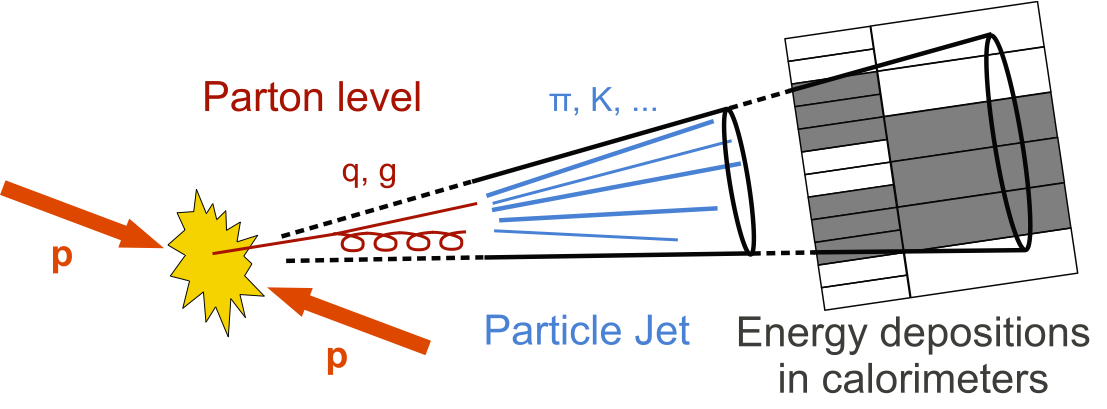
\includegraphics[width=1\linewidth, angle=0]{figs/Objects/jet_schem.png}
  \end{center}
  \caption[A schematic illustrating the formation of hadronic jets and the resulting observed energy deposits in the calorimeter.]
          {A schematic illustrating the formation of hadronic jets and the resulting observed energy deposits in the calorimeter~\cite{obj-jet_schem}.}
  \label{fig:obj-jet_schem}
\end{figure}

This section containts a description of the procedure utilised by ATLAS
to go from energy deposits in calorimeter cells to well defined and calibrated hadronic jets.
This procedure can be split up into three seperate steps that are described in the following sections;
firstly topoclusters are formed as described in Section~\ref{sec:obj-jet_topo},
then jets are formed from topoclusters using reclustering algorithms described in Section~\ref{sec:obj-jet_reco}
and finally Section~\ref{sec:obj-jet_reco} describes how the jets are calibrated and the relevant jet energy uncertainties are derived.

\subsection{Hadronic topocluster reconstruction}
\label{sec:obj-jet_topo}

The first step of jet building at ATLAS builds 3D clusters, known as topoclusters, from neighbouring groups of energy deposits in cells~\cite{obj-jet_topo}.
The calorimter cells can be from either the EM or hadronic calorimeter systems,
which have a dimensions given in Tables~\textbf{LM fix, need to make tables, then reference here}.
The algorithm employed makes use of the variable cell signal significance defined as, 
\begin{equation}
  \Large{S_{\text{cell}}^{EM} = \frac{E_{\text{cell}}^{EM}}{\sigma_{\text{noise,cell}}^{EM}}}
\end{equation}
where $E_{\text{cell}}^{EM}$ is the energy deposited in a cell at the EM-scale \textbf{Laurie fix, check EM scale is defined possibily in detector}
and $\sigma_{\text{noise,cell}}^{EM}$ is the uncertainty due to noise in that cell.
The sources of noise in a calorimeter cell are described in Section \textbf{LM fix, need to have a noise section somewhere...}.
A large value of $S_{\text{cell}}^{EM}$ ( $>$ 1 ) indicates that the energy deposit is likely due to a particle
depositing energy in the calorimeter rather than noise within the calorimeter.

\noindent
Using the value of $S_{\text{cell}}^{EM}$, each calorimeter cell is labelled as follows
\begin{itemize}
\item If $|S_{\text{cell}}^{EM}| > 4$: the cell is labelled a \textbf{seed} cell.
\item If $|S_{\text{cell}}^{EM}| > 2$: the cell is labelled a \textbf{growth} cell.
\item If $|S_{\text{cell}}^{EM}| > 0$: the cell is labelled a \textbf{boundry} cell.
\end{itemize}
Then the algorithms builds clusters as in the following steps,
\begin{enumerate}
\item A seed cell forms the centre of a new topocluster.
\item Neighbouring seed cells are added together to the form one topocluster seed.
\item Then, growth cells neighbouring the topocluster are added.
\item Finally, boundry cells neighbouring the topocluster are added.
\end{enumerate}
Figure~\ref{fig:obj-topo_schem} illustrates an example of where the algorithm would form a topocluster and an example where it wouldn't.

\begin{figure}[!hbt]
  \begin{center}
    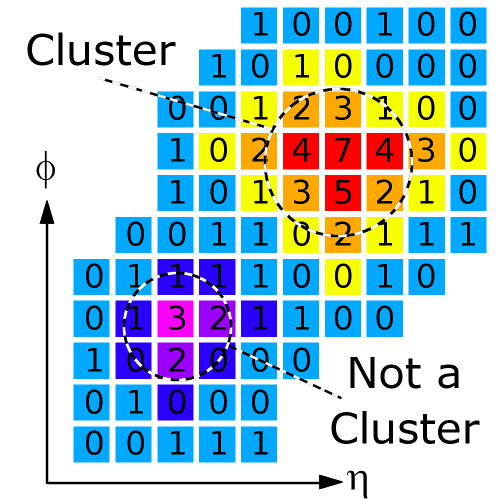
\includegraphics[width=0.6\linewidth, angle=0]{figs/Objects/topo_schem.png}
  \end{center}
  \caption[A schematic illustrating the algorithm used to form a topocluster. The numbers on the grid represent $|S_{\text{cell}}^{EM}|$ and the colours represent the cell label and formed topocluster.]
          {A schematic illustrating the algorithm used to form a topocluster. The numbers on the grid represent $|S_{\text{cell}}^{EM}|$ and the colours represent the cell label and formed topocluster
            ~\cite{det-magnet_fig}.}
  \label{fig:obj-topo_schem}
\end{figure}


\subsection{Jet Reconstruction}
\label{sec:obj-jet_reco}

anti-$k_T$
\subsection{Jet calibration}
(JES, JER, BJES) description

\section{Identification of $b$-jets}
\label{sec:obj-bjets}

Hadronic jets, described in Section~\ref{sec:obj-jets}, can be further categorised into three separate categories based on the flavour of the constituent quarks.
$b$-jets are defined as jets containing one or more $b$-hadrons,
$c$-jets are defined as jets containing one or more $c$-hadrons but no $b$-hadrons
and finally light-flavoured jets comprise of only light hadrons (\textit{u}, \textit{d} and \textit{s} quarks).
A description of how this definition is practically used in simulation is given in Section~\ref{sec:obj-bjet_label}.

The identification $b$-jets, known as $b$-tagging, has been an essential tool in a range of ATLAS collaboration results;
for example analyses studying the $t\bar{t}$ final state \cite{obj-ttbar} \footnote{Section~\ref{sec:trig-sys} contains a concrete example of this.}
and the first direct evidence of the Higgs boson coupling to the quark-sector \cite{obj-Hbb}.
%In the former, as the top decays to a \textit{W}-boson and a $b$-quark with a branching ratio close to 100\%, 
%the application of $b$-tagging can be used increase purity, this is used in the study described in Section~\ref{sec:trig-sys}.
%In the latter, the Higgs boson coupling is proportional to mass squared, hence the large mass of the
%$b$-quark means that $H\to b\bar{b}$ is the decay of the Higgs boson with the largest branching-ratio
%which means that it is the best channel to make the first direct observation of the Higgs boson coupling to fermions.
In the same sense, identification of $b$-jets is an essential part of the analysis being presented here;
by selecting $b$-jets we increase our sensitivity to BSM models that decay to 1 or 2 $b$-jets in their final state.
\textbf{Laurie Fix, link to where I explain why this is good, maybe Intro}.

The process of $b$-tagging at ATLAS in Run-2 has been previously described in great
detail~\cite{obj-bjet_algo_2015,obj-bjet_algo_2016},
so what follows is a summary of the key features of the process.

\subsection{Assigning a Flavour Label}
\label{sec:obj-bjet_label}

In simulation, the particle-level truth information is known, and hence a truth flavour label of a jet can be defined.
Flavour is assigned to jets by matching truth-level heavy-hadrons with $p_{T} >$ 5 GeV and $\Delta R <$ 0.3 between the hadron and the jet.
If a $b$-hadron is matched to a jet, the jet is then declared a $b$-jet;
this process is then repeated for $c$-hadrons and then $\tau$ leptons.
If no match between $b$, $c$ or $\tau$ is achieved then the jet is assigned as a light-flavour jet.
The matching is exclusive, which means that each particle is only assigned to one jet. \textbf{Add a reference, possibly performance}
This definition of truth flavour in simulation is used generally within this thesis.
   
\subsection{Algorithm descriptions}

To identify $b$-jets, $b$-tagging algorithms utilise the long lifetimes of the heavy-hadrons that decay through the flavour changing weak interaction,
a hadron containing a $b$-quark has a lifetime of the order \SI{1.5}{\pico\second} %\cite{obj-bjet_algo_2015}.
A $b$-jet decay chain  will typically contain two of these flavour changing interactions, 
as at the quark level, the $b$-quark contained in the jet will decay to a $c$-quark, which will then decay into a $u$ or $d$ quark.
The long lifetimes of the heavy flavour hadrons means that they will decay a measurable distance from the 
primary vertex, the point where the hard-scatter collision occurs.
Hence, the flavour of a jet can be inferred from the presence of particles
that originate from a point offset from the primary vertex.
In practice this is performed using the topology of tracks formed by the inner detector
and measurements from the calorimeter, which have been described in Section~\ref{sec:det-ID} and \ref{sec:det-calo} respectively.
   
There are three base $b$-tagging algorithms utilised to produce discriminating variables \cite{obj-bjet_algo_2016}, which are described in the next three sections .
%Sections~\ref{sec:obj-bjet_IP}~to~\ref{sec:obj-bjet_JF}.
The variables are then combined in a multi-variate algorithm which is described in Section~\ref{sec:obj-bjet_MV2}.
Figure~\ref{fig:obj_bjet_schem} shows a schematic illustrating how the tracks from the inner detector
are used by the three $b$-tagging algorithms to identify a $b$-jet, the details of this figure are referred to in the following three sections.

\begin{figure}[!htb]
  \begin{center}
    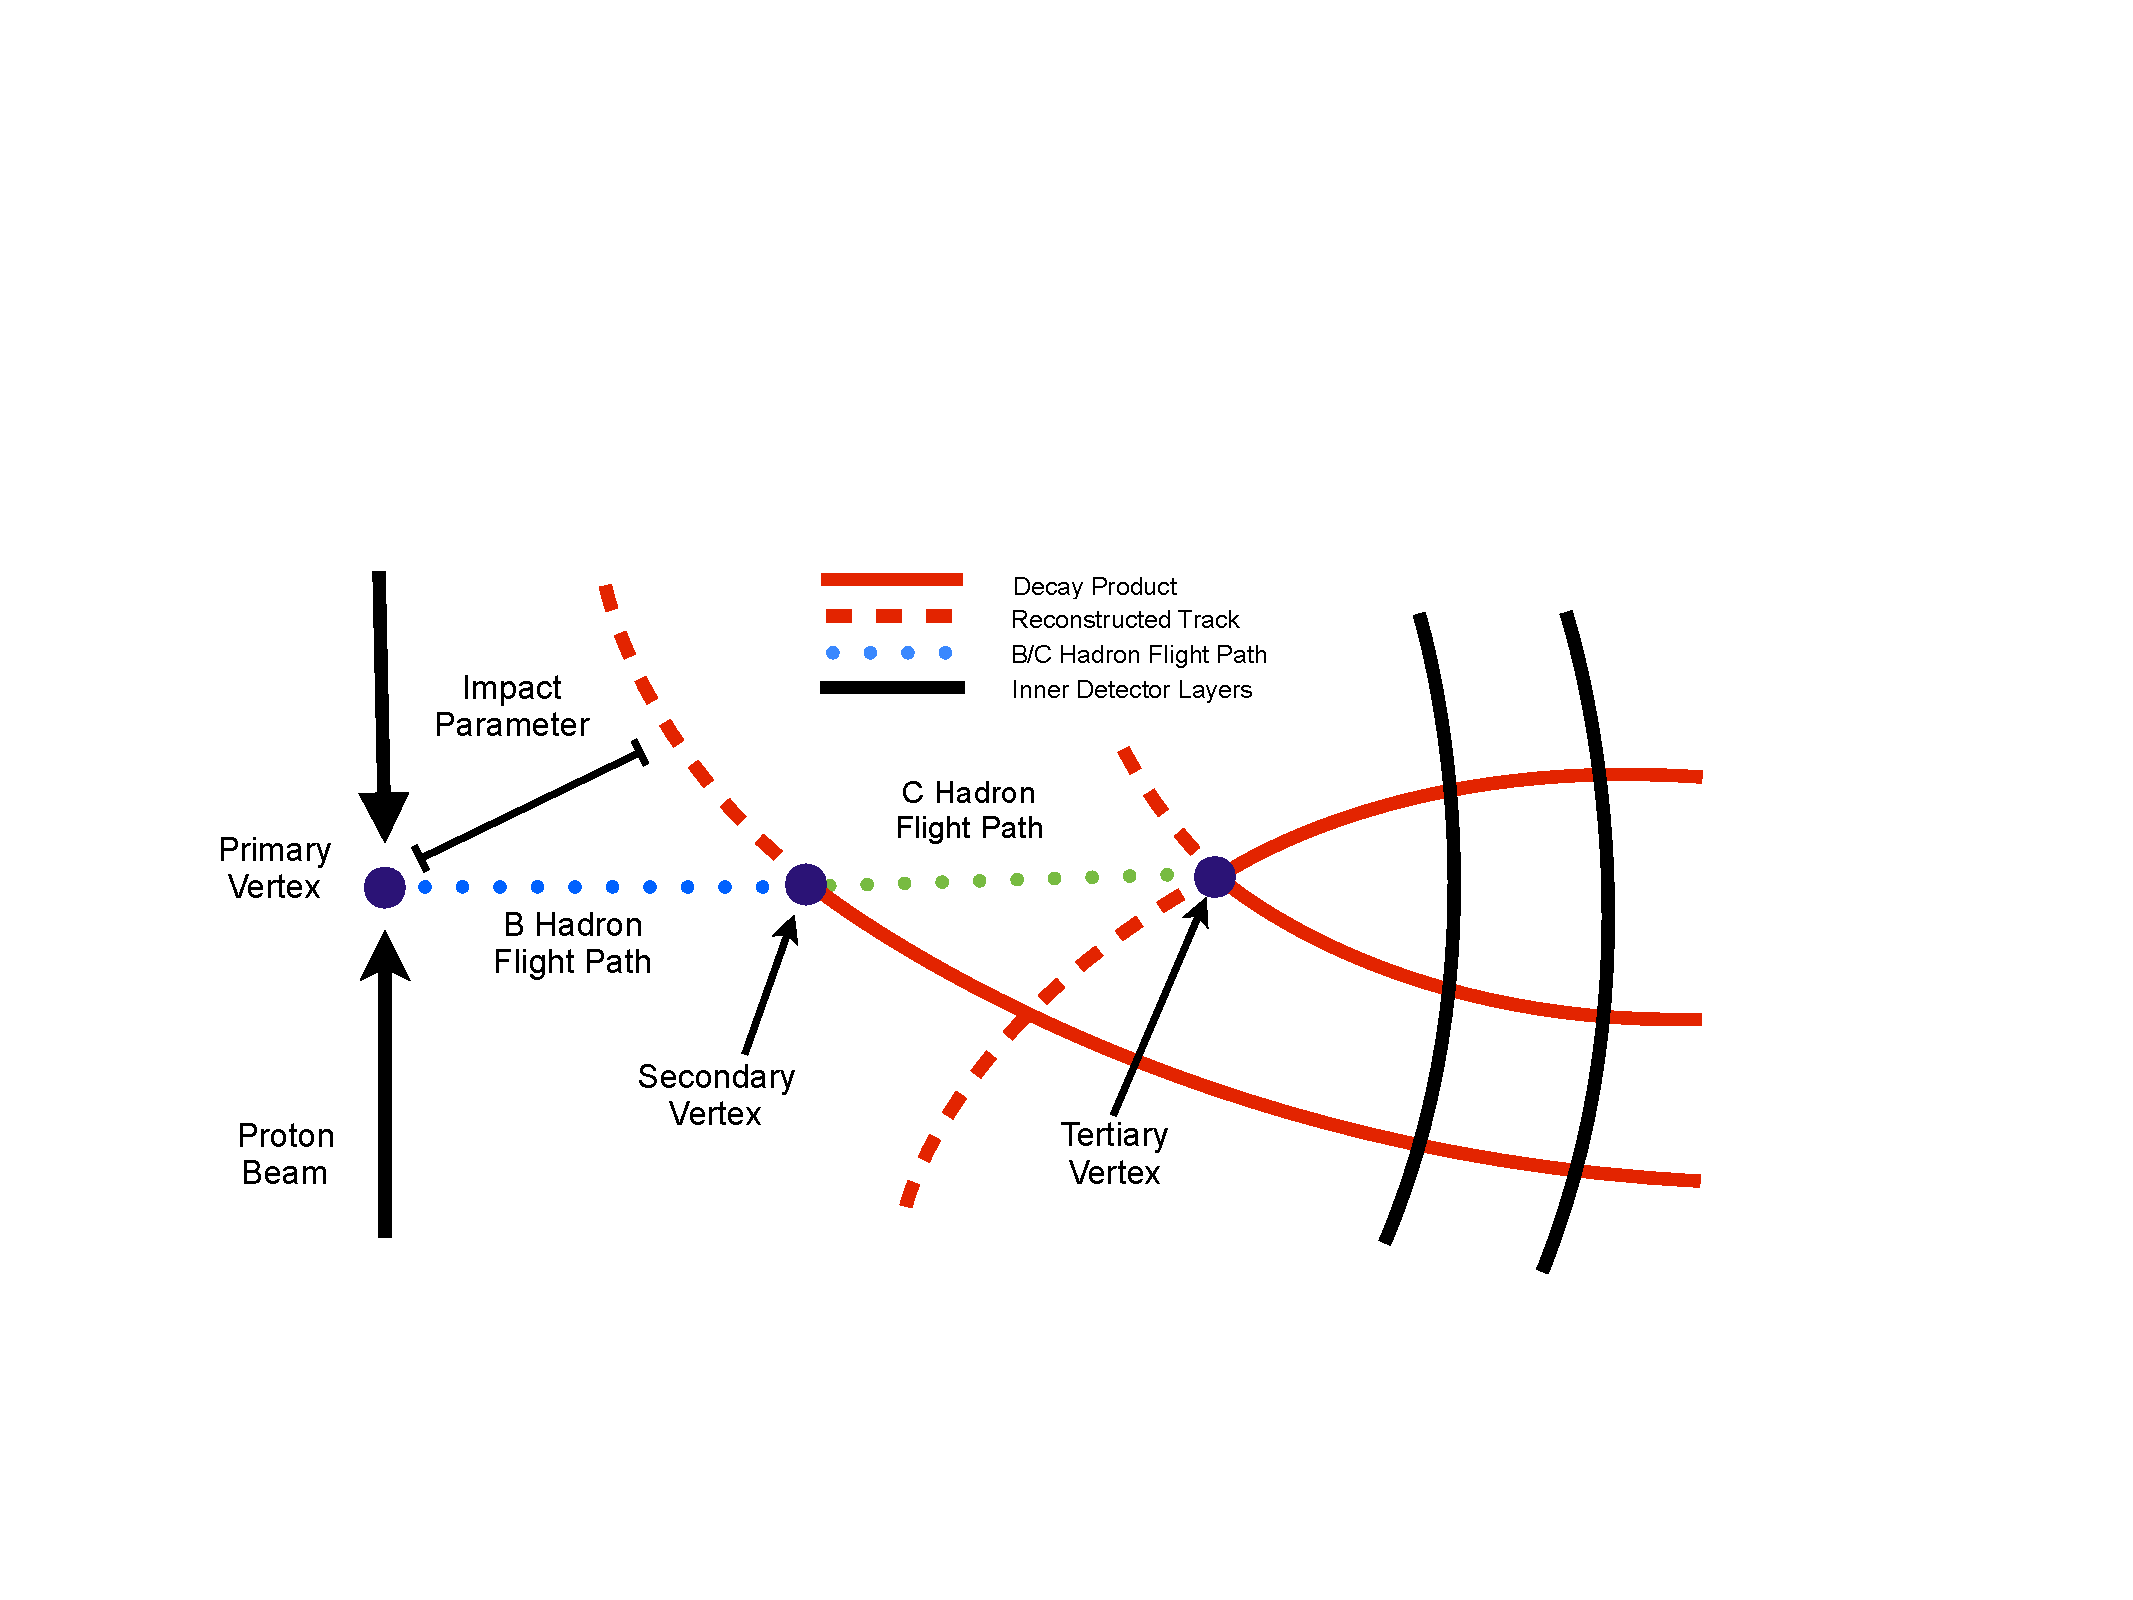
\includegraphics[width=0.9\textwidth]{figs/Objects/bjet_schem.pdf}
    \caption{A diagram to illustrate the key features of a $b$-jet that are utilised by the base $b$-tagging algorithms.}
    \label{fig:obj_bjet_schem}
  \end{center}
  \vspace{-0.5cm}
\end{figure}

\subsubsection{Impact parameter based}
\label{sec:obj-bjet_IP}

The IP3D algorithm is utilises the impact parameter, which is defined as the shortest distance between a specific track and the primary vertex.
A track corresponding to a particle coming from the offset decay vertex of a heavy-hadron is likely to have a large impact parameter,
meaning that the distribution of track impact parameter is different for each of the jet-flavours.
The impact parameter of a track coming from the decay of a heavy hadron is indicated in Figure~\ref{fig:obj_bjet_schem}.
In this algorithm, for all tracks associated to a jet, the impact parameter is calculated in both the transverse (perpendicular to beam-line)
and longitudinal (parallel to beam-line) direction, which are referred to as $d_{0}$ and $z_{0}$.
Then the IP3D algorithm calculates a likelihood of the jet having a specific flavour, 
based on the distributions of the impact parameters ($d_{0}$, $z_{0}$) and their significances 
($d_{0}/\sigma _{d0}$ and  $z_{0}/\sigma_{z0}$) for tracks within the jet. 
Another similar algorithm, IP2D, also calculates the jet flavour likelihood from just the transverse distributions, ($d_{0}$ and $d_{0}$ significance), which is more
robust to pile-up, as tracks from pile-up jets are likely to have a large $z_{0}$ significance value.

\subsubsection{Secondary vertex}
\label{sec:obj-bjet_SV}


The SV1 algorithm aims to reconstruct a secondary vertex of two or more intersecting tracks, corresponding to the decay of a heavy-flavour hadron;
the secondary vertex within a $b$-jet's decay chain is illustrated in Figure~\ref{fig:obj_bjet_schem}.
The SV1 algorithm then calculates many variables that are associated with properties of the reconstructed secondary vertex that show flavour discrimination;
some example variables are the vertex invariant mass,
which will be larger for $b$-jets due to the heavy mass of the $b$-hadron
\footnote{Mass of a B-meson $\sim$ 5 GeV and the mass of a D-meson $\sim$ 1.9 GeV, which are the most common heavy hadrons in a $b$- and $c$-jet respectively.}, 
the distance in the transverse plane between the primary vertex and the secondary vertex, % (2D flight path $L_{XY}$),
which will be larger for $b$-jets due to the long lifetime of the $b$-hadron,
and the number of tracks at the secondary vertex, which will be larger for reliable secondary vertices.

\subsubsection{Jet Fitter}
\label{sec:obj-bjet_JF}

The JetFitter algorithm (JF) attempts to reconstruct the full decay chain of the $b$-hadron into a charmed-hadron and then into light-hadrons. 
This is done by assuming that all vertices lie on a common $b$-flight axis, and then constructing vertices from the intersection of
one or more tracks and the flight axis.
The aim of this is to reconstruct the secondary and tertiary vertices which correspond to the decays of the $b$-hadron and charmed-hadron,
as illustrated in Figure \ref{fig:obj_bjet_schem}.
Similar to SV1, the JetFitter algorithm then calculates a number of flavour discriminating variables:
for example vertex mass and number of vertices with two or more tracks.

\subsubsection{Multi-variate}
\label{sec:obj-bjet_MV2}

The three base algorithms are combined in a boosted decision tree (BDT), a machine-learning technique for combining the many flavour-discriminating variables,
resulting in an algorithm that is known in MV2
As shown in Figure \ref{fig:obj-MV2_schem}, MV2 combines the likelihood output of IP3D and IP2D
with the discriminating variables of SV1 and JF discussed in the preceding sections,
resulting in an output between -1 and 1, where 1 indicates that the jet is likely to be a $b$-jet and -1 indicates the inverse.

\begin{figure}[!htb]
  \begin{center}
    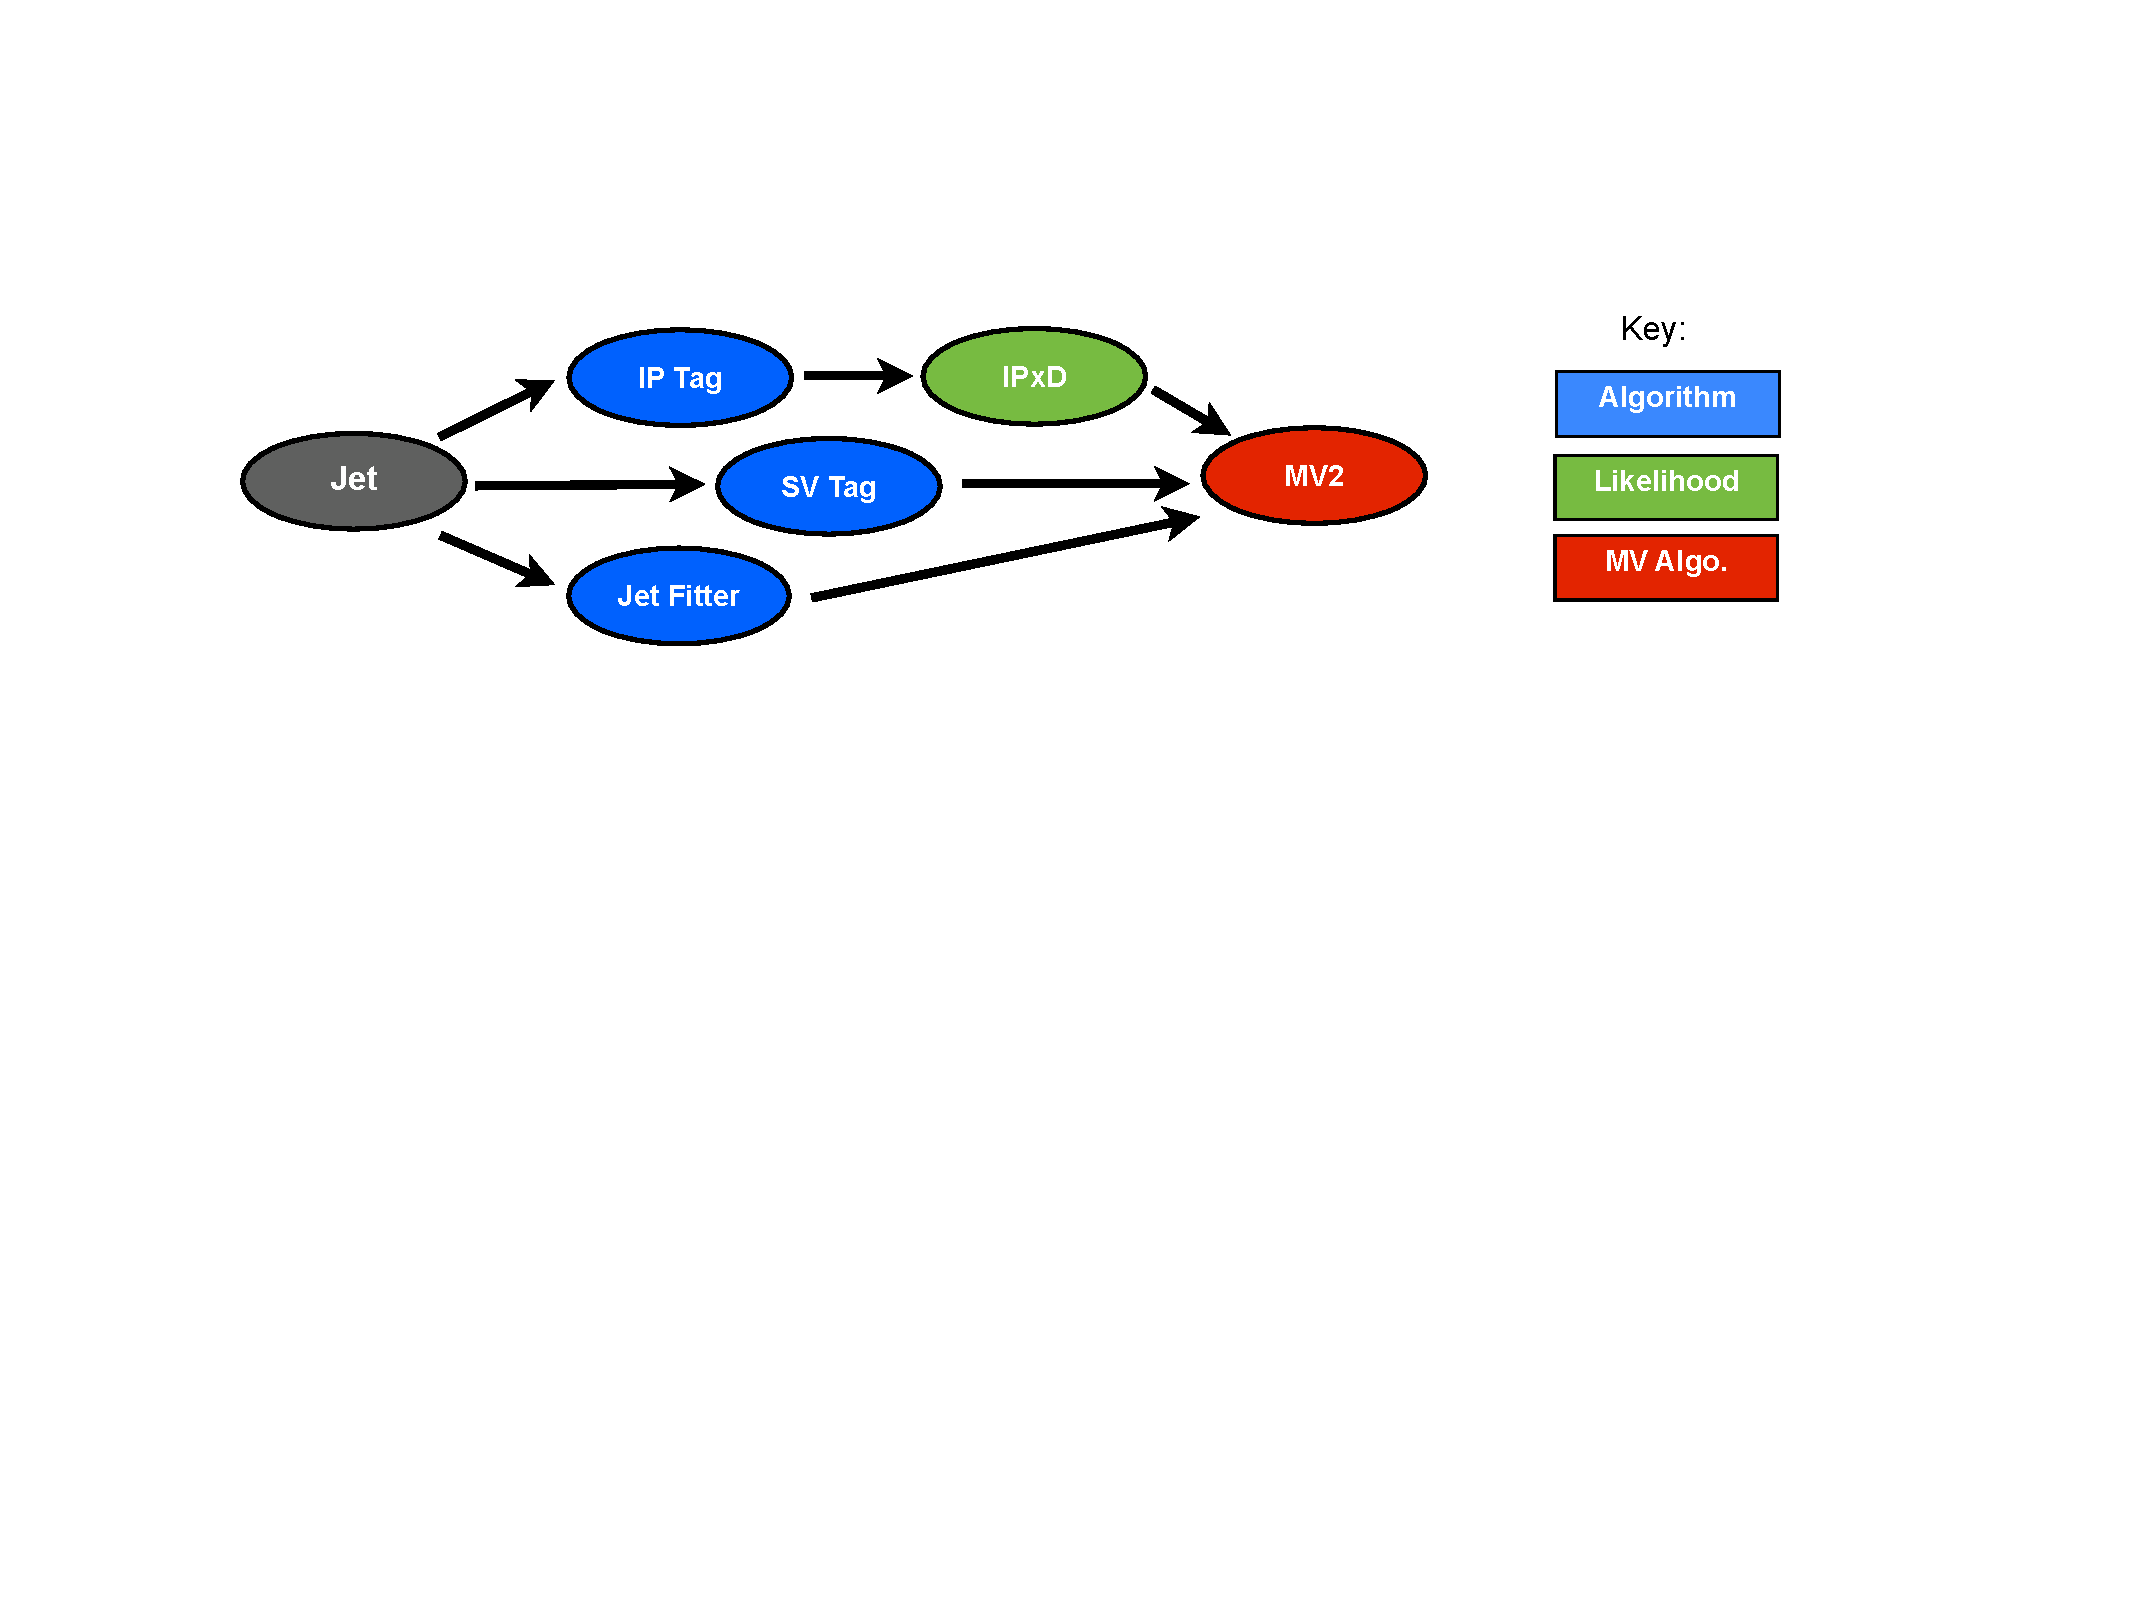
\includegraphics[width=1.0\textwidth]{figs/Objects/MV2_schem.pdf}
    \caption{A diagram illustrating how three base flavour tagging algorithms are combined in the MV2 algorithm.}
    \label{fig:obj-MV2_schem}
  \end{center}
  \vspace{-1cm}
\end{figure}

A cut is then applied to this MV2 output in order to select jets that are likely to $b$-jets.
The cut can be varied to create different operating points which vary the $b$-jet efficiency, light-jet rejection and $c$-jet rejection
\footnote{$b$-jet efficiency is defined as the probability of accepting a true $b$-jet.
  Light-jet rejection is defined as 1 divided by the probability of accepting a true light-jet.
  A similar definition applies for $c$-jet rejection.}.
Looser operating points have a relatively low cut on MV2, meaning that the $b$-jet efficiency is higher at the cost of worse light- and $c$-jet rejections,
and the inverse is true for tighter operating points.
Table~\ref{tab:obj-MV2_WPs} shows the list of fixed cut operating points that are used in ATLAS with a given cut on MV2 output;
shown with the corresponding benchmark $b$-jet efficiency, $c$-jet rejection, light-jet rejection and $\tau$ rejection.
For the remainder of this thesis, the operating points will be referred
\footnote{In this thesis only the fixed-cut operating points shown above will be used,
  however, there also exists a set of flat efficiency operating points where the MV2 cut depends on jet-\pT}
%This is in contrast to the previous multivariate tagger used in Run-1, MV1, which inputted
%the likelihood of a jet having a certain flavour from each of the three base algorithms separately.
\begin{table}[!htb]
  \begin{center}
    \begin{tabular}{|c||c|c|c|c|}
      \hline
      MV2 Cut Value  &  $b$-jet efficiency [\%]  &     $c$-jet rejection   &   Light-jet rejection  &    $\tau$ rejection  \\
      \hline
      0.9349         &           60              &           34          &      1538              &     184              \\
      0.8244         &           70              &           12          &       381              &      55              \\
      0.6459         &           77              &           6           &       134              &      22              \\
      0.1758         &           85              &           3.1         &        33              &     8.2              \\
      \hline
    \end{tabular}
    \caption[The Mv2c10 b-tagging algorithm operating points; with the corresponding $b$-jet~efficiency, $c$-jet~rejection, light-jet~rejection and $\tau$~rejection.]
            {The Mv2c10 b-tagging algorithm operating points; with the corresponding $b$-jet~efficiency, $c$-jet~rejection, light-jet~rejection and $\tau$~rejection.
              This table is taken from reference~\cite{obj-bjet_algo_2016}.}
            \label{fig:obj-MV2_schem}
  \end{center}
  \vspace{-1cm}
\end{table}

The BDT is trained using a simulated sample of $t\bar{t}$ events that will contain a mix of  $b$-, $c$- and light-jets
as well as a sample containing $Z'$ boson decaying to $b$-quarks.
The training makes use of the truth flavour labels assigned to jets using the process described in Section~\ref{sec:obj-bjet_label}.
A training sample with known truth labels is required as this allows the BDT to be optimised
such that it uses the complex correlations between the input variables to allow for high $b$-jet efficiencies
whilst still obtaining a large $c$- and light-jet rejection.
The recommended $b$-tagging tool is MV2c10 which has been trained on a sample containing 10\% charm-jets, to give strong light- and $c$-rejection.

\subsection{Performance}

I have a couple of options here.
=> Put peformance in event selection (tagging efficiency plot)
=> Describe performance here with some discussion of high pT b-Tagging

\section{bTagging: Validation in Dijet Events}

\section{Leptons}   
\subsection{Electron}
\label{sec:obj-electron}
\subsection{Muon}
\label{sec:obj-muon}

